\documentclass[11pt]{article}
\usepackage[small]{titlesec}
\usepackage[top = 0.66in,textwidth = 6.5in, textheight=9.1in]{geometry}

\usepackage{amsmath}
\usepackage{graphicx}
\usepackage{latexsym}
\usepackage{color}
\usepackage{amssymb}
\usepackage{accents}
\usepackage{tabularx}
\usepackage{fancyhdr}
\usepackage{verbatim}
\usepackage{multirow}
\usepackage{framed}
\usepackage{natbib}
\usepackage{float, subfig}
\usepackage{enumitem}
\usepackage{mathtools}
\usepackage{mathrsfs}
\usepackage{amsfonts}
\usepackage{listings}
\usepackage{amsthm}
\usepackage{grffile}
\usepackage{sidecap}
\usepackage{pbox}
\usepackage{algorithm}
\usepackage{longtable}
\usepackage[noend]{algpseudocode}

\def\qed{\hfill{\(\vcenter{\hrule height1pt \hbox{\vrule width1pt height5pt
     \kern5pt \vrule width1pt} \hrule height1pt}\)} \medskip}

\newtheorem{theorem}{Theorem}
\newtheorem{lemma}[theorem]{Lemma}
\newtheorem{corollary}[theorem]{Corollary}
\newtheorem{proposition}[theorem]{Proposition}
\newtheorem{assumption}{Assumption}
\newtheorem{conjecture}[theorem]{Conjecture}
\newtheorem{remark}{Remark}
\newtheorem{example}{Example}
\newtheorem{definition}{Definition}
\renewcommand{\textfraction}{0.0}
\newcommand{\dst}{\displaystyle}
\newcommand{\minx}{\mbox{\( \dst \min_{x \in X} \)}}
\newcommand{\Efx}{\mbox{\( \dst E f (x, \xi) \)}}
\newcommand{\Efxhat}{\mbox{\( \dst E f (\hat{x}, \xi) \)}}
\newcommand{\hxx}{\mbox{\( \hat{x} \)}}
\newcommand{\bpi}{\bar{\pi}}
\newcommand{\xx}{\mbox{\( x \)}}
\newcommand{\txxi}{\mbox{\(\xi\)}}
\newcommand{\var}{\mbox{var}}
\newcommand{\cF}{{\cal F}}
\newcommand{\cG}{{\cal G}}
\newcommand{\cN}{{\cal N}}
\newcommand{\cO}{{\cal O}}
\newcommand{\txi}{{\xi}}
\newcommand{\PP}{\mbox{\(SP\)}}
\newcommand{\PPn}{\mbox{\(SP_n\)}}
\newcommand{\PPnx}{\mbox{\(SP_{n_x}\)}}
\newcommand{\noi}{\noindent}
\renewcommand{\ss}{\smallskip}
\newcommand{\ms}{\medskip}
\newcommand{\bs}{\bigskip}
\newcommand{\st}{\mbox{s.t.}}
\newcommand{\wpo}{\mbox{wp1}}
\newcommand{\iid}{\mbox{i.i.d.\ }}
\newcommand{\vsmo}{\vspace*{-0.1in}}
\newcommand{\vsmt}{\vspace*{-0.2in}}
\newcommand{\vso}{\vspace*{0.1in}}
\newcommand{\vst}{\vspace*{0.2in}}
\newcommand{\mc}{\multicolumn}
\newcommand{\cP}{{\cal P}}
\newcommand{\underv}{\mbox{$\underbar{$v$}$}}
\allowdisplaybreaks 

\renewcommand{\P}{{\mathbb P}}
\newcommand{\E}{{\mathbb E}}
\newcommand{\R}{{\mathbb R}}
\renewcommand{\Re}{{\mathbb R}}
\newcommand{\mbf}{\mathbf}
\renewcommand{\underbar}{\underaccent{\bar}}

\bibliographystyle{plain}

\begin{document}
%0.27
\baselineskip0.25in

\begin{center}
\begin{large}
\begin{bf}

Optimal Crashing of a PERT Network with Disruptions \ms

\today \ms
\end{bf}
\end{large}
\end{center}

\section{Introduction} \label{sec:introduction}
	The management of complex projects through optimization has a rich history in operations research, beginning with the program evaluation and review technique (PERT) \cite{malcolm1959application} and the critical path method (CPM) of \cite{kelley1961criticalpath}; see S{\"o}derlund \cite{soderlund2004building} for an overview and see \cite{Elmaghraby77}. To formulate a mathematical model, a project is viewed as a collection of activities, each of which has some duration and may consume some resources. There are precedence relationships between activities due to logical or technological considerations. The objective is to complete all activities in minimum time. We represent such a project using an acyclic activity network, where the length of each link shows the duration of an activity, and an edge's predecessors capture the precedence relationships. An activity cannot start until all its predecessors are completed. Multiple activities can be processed at the same time without a upper limit, as long as the precedence requirement is satisfied. More details about the activity network are discussed in \cite{Elmaghraby77}.\\
	\newline 
	In the planning stage of a project, decisions are made to crash a certain set of activities in order to minimize the project's timespan. Here crashing an activity means shortening its duration. In this paper, a discrete set of crashing options are available, each with fraction specifying the resulting reduction in the activity's duration. An activity can be crashed at most once and with a single option. Each option incurs a certain cost, and the total cost of crashing cannot exceed the budget. Optimization of such static crashing problems is introduced in \cite{fulkerson1961network, kelley1961criticalpath}. Under a finite set of crashing options, the problem can be modeled as a mixed integer program. The static model can be extended to incorporate uncertainty of activity durations. Monte Carlo simulation methods are used to estimate the expected project span given distributions of activity lengths, since it is is difficult to express analytically the expected project span \cite{burt1971conditional,van1963letter}. Heuristics and simulation-based algorithms have been developed to solve the stochastic project crashing problem \cite{aghaie2009ant,bowman1994stochastic,ke2014genetic,kim2007heuristic}. Another approach to handle the uncertainty is robust optimization, in which the objective is to minimize the worst case project span within a specified uncertainty set. While affinely adaptive recourse decisions are computationally tractable as linear, or second-order cone, programs, this restriction may lead to suboptimal solutions \cite{chen2008linear,cohen2007stochastic}. However, once recourse decisions can take general form, the robust model is only tractable with hypercube uncertainty sets, which is a trivial case because the worst-case scenario in the uncertainty set is always the point where every activity takes its upper bound \cite{wiesemann2012robust}. Ahipasaoglu et al. \cite{ahipasaoglu2016distributionally} propose a distributionally robust optimization scheme applied to a PERT network, which reformulates the problem as a semidefinite program or a copositive program, depending on the description of uncertainty.\\
	\newline
	The uncertainty in our paper lies in the timing and the magnitude of the stochastic disruption, which is modeled differently from randomness in a two-stage stochastic program or from the uncertainty set in robust optimization. A stochastic disruption is an event that may occur any time in the time horizon and change the system parameters significantly. A few authors apply this idea when the disruption can only occur in a set of specified time periods. Yu and Qi \cite{yu2004disruptionmgt} introduce scenario-based optimization models for airline scheduling. Morton et al. \cite{morton2009sealift} introduce a sealift scheduling problem under a finite number of stochastic disruptions within a stochastic programming structure. This structure ``falls between standard two-stage and multi-stage stochastic programs for a multi-period problem" and reduces the size of the problem to a quadratic growth in the number of time periods. Our setting inherits the philosophy of \cite{morton2009sealift} but enhances the model by allowing a continuous disruption time instead of a prespecified set of fixed time periods. \\
	\newline
	We first formally describe the crashing optimization problem under stochastic disruptions. Given a limited number of disruption scenarios, the problem can be formulated as a stochastic mixed integer program and we present the extensive formulation in Section~\ref{sec:formulation}. If we assume a continuous distribution for the disruption time and magnitude, a sample average approximation (SAA) can be used to create a finite set of scenarios and approximate the original problem by a finite-sized optimization problem. We present some important properties of this problem using a serial activity network as a special case in Section~\ref{sec:examples}. 
	\begin{comment}
	We prove some important consistency and convergence properties of the SAA problem using independent and identically distributed samples and stratified samples in Section~\ref{sec:consistency}.\\
	\newline
	The large scale and the discrete non-convex nature of the SAA problem's extended formulation means it may not be solved efficiently to desirable tolerance level. In Section~\ref{sec:decomposition}, a branch-and-cut method based on Benders decomposition is developed to solve the crashing optimization problem with a disruption. We show such a decomposition method solves the integer program to the exactness within finite number of iterations.\\
	\newline
	The experiment results are presented in Section~\ref{sec:results}, including the comparison between the quality of our solution and the solution obtained by solving a  crashing optimization problem with a deterministic disruption, and the computational performance of the decomposition method in Section~\ref{sec:decomposition}, compared to that of solving the extensive formulation. We conclude our paper with remarks on potential extensions of this model in Section~\ref{sec:conclusions}.
	\end{comment}
	
\section{Problem Formulation} \label{sec:formulation}
	The deterministic project crashing optimization problem has been known since the 1960s \cite{fulkerson1961network, kelley1961criticalpath}. Suppose the activity network is represented by a directed graph \(\mathcal{G} = (I,\mathcal{A})\), where the set of activities is denoted by \(I\) and their precedence relationship is characterized by \(\mathcal{A}\). The arc \((i,j) \in \mathcal{A}\) indicates that activity \(i\) has to be finished before the start of activity \(j\). We create two dummy activities \(S\) and \(T\) to represent the start and the end of entire project. \(S\) should precede every activity \(i \in I \backslash \{S\}\) and \(T\) should succeed every activity \(i \in I \backslash \{T\} \). \\
	\newline
	For each activity \(i \in I\), the nominal length \(D_i\) is given. We can apply a finite set of crashing options, \(j \in J_i\), and one unit application of each option incurs a cost of \(b_{ij}\), while it decreases the length of activity \(i\) by \(D_ie_{ij}\). The total cost of crashing options cannot exceed a given budget, \(B\). We assume each activity can be crashed at most with one unit and the problem can be formulated as follows:
	\begin{subequations} \label{prob:static}
		\begin{align}
		\min \quad & t_T &\\
		\text{s.t.} \quad &  t_k - t_i \geq D_{i}(1 - \sum_{j \in J_i} x_{ij} e_{ij}) \qquad \qquad \forall \,i \in I, (i,k) \in \mathcal{A} \label{cons:dSep}\\
		& \sum_{i \in I} \sum_{j \in J_i} b_{ij}x_{ij} \leq B  \label{cons:dBudget}\\
		& \sum_{j \in J_i} x_{ij} \leq 1  \qquad \qquad \forall \,i \in I \label{cons:dSingleBudget}\\
		& t_i \geq 0  \qquad \qquad \forall \,i \in I\\
		& 0 \leq x_{ij} \leq 1  \qquad \qquad \forall \,i \in I, j \in J_i.
		\end{align}
	\end{subequations}
	In this formulation, \(t_i\) represents the starting time of activity \(i \in I\). We aim to minimize the project span, which is the starting time of the terminal activity, \(t_T\). Constraint~\eqref{cons:dSep} guarantees the precedence relationship: if activity \(i\) precedes activity \(k\), activity \(k\) cannot start until activity \(i\) is finished, since the finishing time of activity \(i\) is \(t_i + D_i (1- \sum_{j \in J_i} x_{ij}e_{ij})\). Constraint~\eqref{cons:dBudget} is the budget constraint and constraint~\eqref{cons:dSingleBudget} ensures that no more than one unit of crashing option can be applied to an activity. \\
	\newline
	In our problem, we assume at most one stochastic disruption can occur at a random time in the project span. We also assume for each activity \(i \in I\), the crashing decision for that activity needs to be made at the start of that activity, and cannot be changed afterwards. The disruption does not affect the started activities but changes the length of those that have not started according to a random distribution. It is usually hard to compute the recourse function directly when parameters are distributed according to continuous distributions, and therefore SAA is proposed to approximate the problem by a large-scale deterministic optimization problem with a finite scenario set \cite{kim2015guide,shapiro2009lectures}. In this paper, we assume there is a discrete finite set of scenarios indexed by \(\omega \in \Omega\). For each scenario \(\\omega\), the random realization of parameters, \(\xi^\omega\), consists of the timing of disruption, \(H\), and the changed duration of each activity, \(d_i, \forall i \in I\). \\
	\newline
	If there is at most one disruption, we can model the problem as a two-stage stochastic mixed integer program. The definition of our first stage is different from the traditional stochastic program setting. Here the first stage contains decisions through completion of the project if no disruption occurs and the second stage characterizes the decisions for each realization of the disruption. This means that the first stage decision variables are carried out until the disruption, if it ever occurs, and after the disruption, the scenario-specific recourse decisions are executed.\\
	\newline
	The notation for the model is displayed as follows:
	\begin{longtable}[H]{ l l l l }
		\multicolumn{4}{l}{Indices and index sets} \\
		\\
		\(I\) & \(\qquad\) & the set of activities;&\\
		\(J_i\) & \(\qquad\) & the set of crashing options for activity \(i\), \(i \in I\);&\\
		\(\Omega\) & \(\qquad\) & the index set of possible realizations of disruption;&\\
		\(\mathcal{A}\) &\(\qquad\) & set of arcs which represents the precedence relationship;&\\
		\\
		\multicolumn{4}{l}{Parameters} \\
		\\
		\(D_{i}\)& \(\qquad\) & original duration of activity \(i\), \(i \in I\);&\\
		\(e_{ij}\) & \(\qquad\) & effectiveness of crashing option \(j\), \(i \in I, j \in J_i\);&\\
		\(B\) & \(\qquad\) & total budget;&\\
		\(b_{ij}\) & \(\qquad\) & cost of crashing option \(j\), \(i \in I, j \in J_i\);&\\
		\(H^\omega\) &\(\qquad\) & disruption time in scenario \(\omega\), \(\omega \in \Omega\);&\\
		\(d_{i}^\omega\) & \(\qquad\)&the change of duration of activity \(i\) in realization \(\omega\), &\\
		& \(\qquad\) & if the activity is started after the disruption, \(i \in I, \omega \in \Omega\);& \\
		\(p^\omega\) & \(\qquad\) & the probability of scenario \(\omega\), \(\omega \in \Omega\);& \\
		\(p^0\) & \(\qquad\) & the probability of no disruption;& \\
		\\
		\multicolumn{4}{l}{Decision Variables}\\
		\\
		\(t_{i}\) & \(\qquad\) & nominal starting time of activity \(i\), \(i \in I\);&\\
		\(x_{ij}\) & \(\qquad\) & fraction activity \(i\) is crashed by option \(j\) in the nominal plan, \(i \in I, j \in J_i\); &\\
		\(t_{i}^\omega\) & \(\qquad\) & starting time of activity \(i\) under scenario \(\omega\), \(i \in I, \omega \in \Omega\);&\\
		\(x_{ij}^\omega\) & \(\qquad\) & fraction activity \(i\) is crashed by option \(j\) under scenario \(\omega\), \(i \in I, j \in J_i, \omega \in \Omega \); &\\
		\(G_i^\omega\) & \(\qquad\) & indicator whether activity \(i\) starts after disruption in realization \(\omega\), \(i \in I, \omega \in \Omega\);&\\
		\(z_{ij}^\omega\) & \(\qquad\) & binary term to linearize the bilinear term \(G_i^\omega x_{ij}^\omega\), \(i \in I, j \in J_{i}, \omega \in \Omega\).&\\
	\end{longtable}
	\noi The extensive formulation of the two-stage stochastic program is shown as formulation~\eqref{prob:extensive}:
	\begin{subequations} \label{prob:extensive}
		\begin{align}
		\min \quad & p^0 t_T + \sum_{\omega \in \Omega} p^\omega t_T^\omega \\
		\text{s.t.} \quad & t_k - t_i \geq D_{i}(1 - \sum_{j \in J_i} x_{ij} e_{ij}) \qquad \qquad \forall \,i \in I, (i,k) \in \mathcal{A} \label{cons:Sep}\\
		& \sum_{i \in I} \sum_{j \in J_i} b_{ij}x_{ij} \leq B  \label{cons:Budget}\\
		& \sum_{j \in J_i} x_{ij} \leq 1  \qquad \qquad \forall \,i \in I \label{cons:SingleBudget}\\
		& H^\omega + G_i^\omega M \geq t_i \qquad \qquad \forall \,i \in I, \omega \in \Omega \label{cons:G1}\\
		& H^\omega - (1 - G_i^\omega) M \leq t_i \qquad \qquad \forall \,i \in I, \omega \in \Omega \label{cons:G2}\\
		& t_i^\omega + G_i^\omega M_t \geq t_i \qquad \qquad \forall \,i \in I, \omega \in \Omega \label{cons:tG1}\\
		& t_i^\omega - G_i^\omega M_t \leq t_i \qquad \qquad \forall \,i \in I, \omega \in \Omega \label{cons:tG2}\\
		& x_{ij}^\omega + G_i^\omega \geq x_{ij} \qquad \qquad \forall \,i \in I, j \in J_i, \omega \in \Omega \label{cons:xG1}\\
		& x_{ij}^\omega - G_i^\omega \leq x_{ij} \qquad \qquad \forall \,i \in I, j \in J_i, \omega \in \Omega \label{cons:xG2}\\
		& t_k^\omega - t_i^\omega \geq D_i + d_i^\omega G_i^\omega -\sum_{j \in J_i} D_i e_{ij} x_{ij}^\omega - \sum_{j \in J_i} d_i^\omega e_{ij} z_{ij}^\omega \qquad \qquad \forall \,i \in I, j \in J_i, \omega \in \Omega \label{cons:scenSep}\\
		& \sum_{j \in J_i} x_{ij}^\omega \leq 1 \qquad \qquad \forall \,i \in I, \omega \in \Omega \label{cons:scenBudget1}\\
		& \sum_{i \in I}\sum_{j \in J_i} b_{ij}x_{ij}^\omega \leq B \qquad \qquad \forall \,\omega \in \Omega \label{cons:scenBudget}\\
		& z_{ij}^\omega \leq G_i^\omega \qquad \qquad \forall \,i \in I, j \in J_i, \omega \in \Omega \label{cons:linearize1}\\
		& z_{ij}^\omega \leq x_{ij}^\omega \qquad \qquad \forall \,i \in I, j \in J_i, \omega \in \Omega \label{cons:linearize2}\\
		& z_{ij}^\omega \geq G_i^\omega + x_{ij}^\omega - 1 \qquad \qquad \forall \,i \in I, j \in J_i, \omega \in \Omega \label{cons:linearize3}\\
		& t_i \geq 0 \qquad \qquad \forall \,i \in I \label{cons:nonnegt}\\
		& t_i^\omega \geq H^\omega G_i^\omega \qquad \qquad \forall\, i \in I, \omega \in \Omega \\
		& 0 \leq x_{ij} \leq 1 \qquad \qquad \forall \,i \in I, j \in J_i\\ 
		& 0 \leq x_{ij}^\omega \leq 1 \qquad \qquad \forall \,i \in I, j \in J_i, \omega \in \Omega\\
		& 0 \leq z_{ij}^\omega \leq 1 \qquad \qquad \forall \,i \in I, j \in J_i, \omega \in \Omega\\
		& G_i^\omega \in \{0,1\}. \qquad \qquad \forall \,i \in I, \omega \in \Omega.
		\end{align}
	\end{subequations}
	In model~\eqref{prob:extensive}, we are minimizing the expected project span by taking the sum of each scenario's project span weighted by the scenario probability. We keep the constraints~\eqref{cons:dSep}-\eqref{cons:dSingleBudget} for the nominal scenario as~\eqref{cons:Sep}-\eqref{cons:SingleBudget}. In constraints~\eqref{cons:G1}-\eqref{cons:G2}, variables \(G^\omega_i\) takes value \(1\) if activity \(i\) starts after the disruption time; otherwise it takes value 0, and \(M\) is a large number to enforce this logic relationships. This is important in our problem setting because the duration of each activity depends on its temporal relationship to the disruption time, which is reflected in constraint~\eqref{cons:scenSep}. Also we have to ensure that the decisions made before the disruption time in each scenario are the same as the nominal decisions. Therefore, we set up non-anticipativity constraints~\eqref{cons:tG1}-\eqref{cons:xG2}. For each scenario, the duration of activity \(i\) becomes \((D_i + d_i^\omega G_i^\omega)(1 - \sum_{j \in J_i} e_{ij}x_{ij}^\omega)\), which expands to the form of constraint~\eqref{cons:scenSep}. If \(G_i^\omega = 0\), which means activity \(i\) starts before the disruption time of scenario \(\omega\), this expression is the same as \(D_i (1 - \sum_{j \in J_i} e_{ij}x_{ij})\) since \(x_{ij} = x_{ij}^\omega\) is enforced by constraints~\eqref{cons:xG1} and~\eqref{cons:xG2}. If \(G_i^\omega = 1\), then the duration of activity \(i\) is changed to \(D_i + d_i^\omega\). The expression \((D_i + d_i^\omega G_i^\omega)(1 - \sum_{j \in J_i} e_{ij}x_{ij}^\omega)\) contains a bilinear term \(G_i^\omega x_{ij}^\omega\), which can be linearized by introducing a binary variable \(z_{ij}^\omega\) and constraints \eqref{cons:linearize1}-\eqref{cons:linearize3}.
	
\section{Illustration of Problem Properties via Examples} \label{sec:examples}
	In this section we show a serial example to illustrate the nature of the project crashing problem under stochastic disruption, which is different from the deterministic problem. In the deterministic project crashing problem, all activities on the critical path should start as soon as possible. However, with a stochastic disruption, it might be optimal to delay the start of some activities. Therefore, it is necessary to have decision variable \(t_i, \forall i \in I\) in model~\eqref{prob:extensive} in addition to the crashing decision variable \(x_{ij}, \forall i \in I, j \in J_i\). \\
	\newline
	It is obvious that the delay can possibly be beneficial if \(d_i^\omega < 0\) for some \(i \in I\) and \(\omega \in \Omega\). We use a serial activity network to show the possibility of beneficial delay, even if all activities are lengthened by the disruption, a.k.a., \(d_i^\omega > 0, \forall i \in I, \omega \in \Omega\). Suppose we have a project with three activities in a serial network form. Activity 1 must finish before the start of activity 2 and the activity 2 must finish before the start of activity 3. The structure of the project is displayed as follows. We add a dummy activity ``T" to represent the end of the project. The total crashing budget is \(1\). 
	\begin{figure}[H]
		\centering
		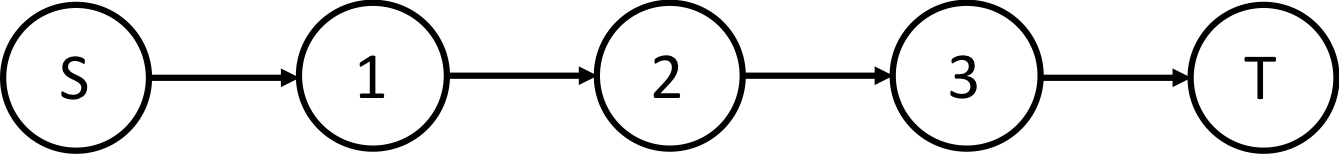
\includegraphics[width=0.8\textwidth]{serial3}
		\caption{Example of a 3-activity project}
		\label{fig:serial3}
	\end{figure}
	\noi In this example, \(I=\{1,2,3,T\}\), \(D_1=9\), \(D_2=10\), and \(D_3=7\). There is only one crashing option for each activity, so we omit the subscript to index the crashing options. We use \(e_i = 0.5\) for all \(i \in I\). The probability of the disruption not occurring is \(p^0=\frac{1}{2}\), and if a disruption occurs, it will occur at the time \(H^2 = 9.1\). The set of scenario \(\Omega = \{1\}\), where scenario 1 represents the disruption scenario. Suppose the disruption does not affect activity 1, \(d_1^1 = 0\), increases the duration of activity 2 by \(0.1\), \(d_2^1 = 0.1\), and increases the duration of activity 3 by \(6\), \(d_3^1 = 6\). We can see it is optimal to delay the start of activity 2 to \(t_2 = 9.1\). There we are able to observe whether the disruption happens. If the disruption occurs, it is optimal to spend the entire budget to crash activity 3, and otherwise it is optimal to crash activity 2 with \(1\) amount of resource. The expected total project span is \(23.4\), as the optimal project span given no disruption is \(21.1\) and that under disruption is \(25.7\). If every activity starts as soon as possible, like in the deterministic problem, we cannot observe whether the disruption happens or not prior to the start of activity 2. Under this condition, the best solution is to crash activity 2 with \(1\) amount of crashing resource, and the optimal expected project span is \(24\), larger than \(23.4\). \\
	\newline
	Because it is possible for an optimal crashing plan to contain a delay for some activities, we have to set up decision variables \(t_i,\ \forall i \in I\), as the starting time of each activity, rather than assume that each activity starts as soon as all of its predecessors are finished.  We summarize the reasons of such delay include:
		\begin{enumerate}
			\item Some activities might have a shorter length after disruption. It is beneficial to wait a short period of time to capture this advantage.
			\item Even if all possible disruption magnitudes are adverse, which means they lengthen all activities, it is beneficial to delay an activity so that the crashing resource could be optimally applied according to the realization of disruption.
		\end{enumerate}
	In addition, under a stochastic disruption, it is possible that on a critical path, an activity with a smaller expected length is crashed with a larger amount of resource, while in the deterministic case, it is always optimal to start crashing from the longest one on the critical path. We present a following example to showcase this property. Suppose we have a two-activity serial network, and the disruption time follows a probability distribution shown in Figure~\ref{fig:2act}. The nominal durations of two activities are \(D_1 = 3, D_2 = 4\). The disruption does not affect the duration of activity 1, as \(d_1 = 0\), and lengthens the activity 2 by a random variable distributed in a uniform distribution with upper bound \(10\) and lower bound \(0\), as \(d_2 \sim \mathcal{U}(0,10)\). The crashing option setting is the same as the previous example, as there is only one crashing option for each activity and \(e_i = 0.5, \forall i \in I\). The total budget \(B = 1\).
		\begin{figure}[H]
			\centering
			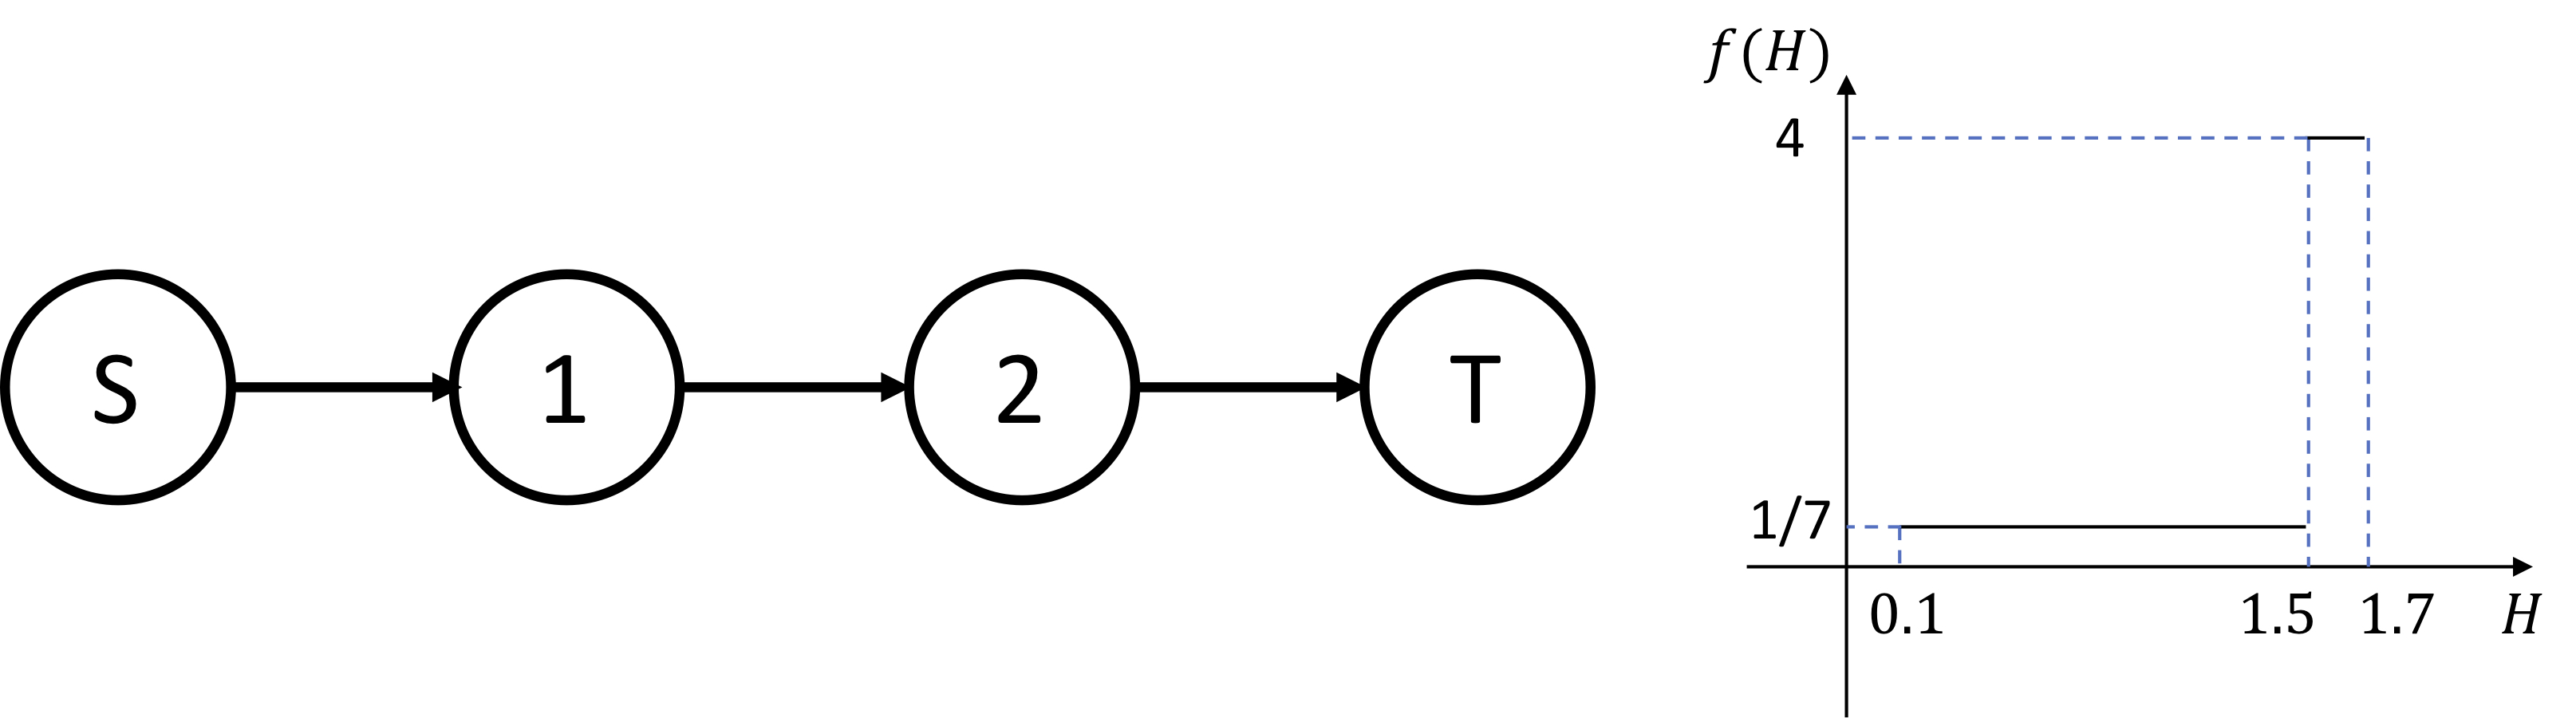
\includegraphics[width=0.8\textwidth]{2act}
			\caption{Left: an illustration of a 2-activity project; right: probability distribution function of disruption time.}
			\label{fig:2act}
		\end{figure}
	\noi In this example, the optimal solution is to crash activity 1 with one unit of resource, i.e.\,\(x_1 = 1, x_2 = 0\). Activity 1 starts at time \(t_1 = 0\) and activity 2 starts at time \(t_2 = 1.5\). The optimal expected project span is \(\mathbb{E}[t_T] = 6.5\). We can compare an alternative solution which crash activity 2 with one unit of resource, which has a longer expected duration. Crashing activity 2 matches the intuition from the deterministic case where on the critical path the activities with longer expected duration are prioritized. However, in this case with a stochastic disruption, the latter solution (\(t_1 = 0, t_2 = 3, x_1 = 0, x_2 = 1\)) yields a longer expected project span as \(\mathbb{E}[t_T] = 7.5\). The reason behind this gap is that by crashing activity 1 with one unit amount of resource, the probability of activity 2 starting before the disruption increases to \(0.8\), which prevents activity 2 from seeing the increased duration. \\
	\newline
	These examples above indicate that the crashing optimization problem with stochastic disruption has complicated nature. The intuition of deterministic crashing optimization problem does not apply here, and we need a math program model as~\eqref{prob:extensive} to solve for the best crashing plan.
	\textcolor{blue}{NP-hardness proof. Add the conclusion of consistency. Add the proof of consistency. Prove the inconsistency of the stratified sampling method. }
	
	\section{Decomposition Method} \label{sec:decomposition}
	Model~\eqref{prob:extensive} is a two-stage stochastic mixed integer program (2SMIP). If we attempt to decompose it into a master problem~\eqref{prob:masterOri} and scenario-specific subproblems~\eqref{prob:subOri}, the state variables \(t\) and \(x\) are all continuous and binary variables exist in the recourse problems. The recourse problems become nonconvex. Most of previous literature of stochastic mixed integer programming assumes a special structure or property which cannot be applied to our problem setting. \textcolor{blue}{For example, Sherali/Fracticelli, Sen/Higle, Ntaimo/Sen, Sherali/Zhu, Sen/Sherali, Gade/Kucukyavuz/Sen solve 2SMIPs with pure binary first stage variables using sequential convex approximation of recourse by a branch-and-cut process framework where disjunctive cuts or Gomory cuts are added. Ahmed/Sun/Zou assumes state variables to be binary so that the Lagrangian cuts are a tight approximation of the recourse function. Caroe/Tind solves a more general case of 2SMIP by using the MIP duality theory but the practical tractability is not optimistic. }
	\begin{subequations}
		\label{prob:masterOri}
		\begin{align}
		(M) \quad z^* = \min \quad &p^0 t_T + \sum_{\omega \in \Omega} p^\omega f^\omega(t,x)\\
		\text{s.t.} \quad & t_k - t_i \geq D_{i}(1 - \sum_{j \in J_i} x_{ij} e_{ij}) \qquad \qquad \forall \,i \in I, (i,k) \in \mathcal{A} \label{cons:MSep}\\
		& \sum_{i \in I} \sum_{j \in J_i} b_{ij}x_{ij} \leq B  \label{cons:MBudget}\\
		& \sum_{j \in J_i} x_{ij} \leq 1  \qquad \qquad \forall \,i \in I \label{cons:MSingleBudget}\\
		& t_i \geq 0 \qquad \qquad \forall \,i \in I\\
		& 0 \leq x_{ij} \leq 1 \qquad \qquad \forall \,i \in I, j \in J_i.
		\end{align}
	\end{subequations}
	\begin{subequations}
		\label{prob:subOri}
		\begin{align}
		(S^\omega) \qquad f^\omega(\hat{t},\hat{x}) = \min \quad & t_T \\
		& H^\omega + G_i M \geq \hat{t}_i \qquad \qquad \forall \,i \in I \label{cons:sG1}\\
		& H^\omega - (1 - G_i) M \leq \hat{t}_i \qquad \qquad \forall \,i \in I \label{cons:sG2}\\
		& t_i + G_i M_t \geq \hat{t}_i \qquad \qquad \forall \,i \in I \label{cons:stG1}\\
		& t_i - G_i M_t \leq \hat{t}_i \qquad \qquad \forall \,i \in I \label{cons:stG2}\\
		& x_{ij} + G_i \geq \hat{x}_{ij} \qquad \qquad \forall \,i \in I, j \in J_i \label{cons:sxG1}\\
		& x_{ij} - G_i \leq \hat{x}_{ij} \qquad \qquad \forall \,i \in I, j \in J_i \label{cons:sxG2}\\
		& t_k - t_i \geq D_i + d_i^\omega G_i -\sum_{j \in J_i} D_i e_{ij} x_{ij} - \sum_{j \in J_i} d_i^\omega e_{ij} z_{ij} \nonumber \\ 
		& \qquad \qquad \forall \,i \in I, j \in J_i \label{cons:subSep}\\
		& \sum_{j \in J_i} x_{ij} \leq 1 \qquad \qquad \forall \,i \in I \label{cons:subBudget1}\\
		& \sum_{i \in I}\sum_{j \in J_i} b_{ij}x_{ij} \leq B \qquad \qquad \forall \,\omega \in \Omega \label{cons:subBudget}\\
		& z_{ij} \leq G_i \qquad \qquad \forall \,i \in I, j \in J_i \label{cons:sublinearize1}\\
		& z_{ij} \leq x_{ij} \qquad \qquad \forall \,i \in I, j \in J_i \label{cons:sublinearize2}\\
		& z_{ij} \geq G_i + x_{ij} - 1 \qquad \qquad \forall \,i \in I, j \in J_i \label{cons:sublinearize3}\\
		& t_i \geq H^\omega G_i \qquad \qquad \forall\, i \in I \label{cons:subH}\\
		& 0 \leq x_{ij} \leq 1 \qquad \qquad \forall \,i \in I, j \in J_i\\
		& 0 \leq z_{ij} \leq 1 \qquad \qquad \forall \,i \in I, j \in J_i\\
		& G_i \in \{0,1\}. \qquad \qquad \forall \,i \in I. \label{cons:subInt}
		\end{align}
	\end{subequations}
	We can relax the integrality constraints~\eqref{cons:subInt} and solve the subproblem to obtain Benders' cuts. Although those Benders' cuts are no longer a tight approximation of the recourse function \(f^\omega(x,t), \forall \omega \in \Omega\), they still provide a valid lower bound. On the other hand, in each iteration of the Benders' decomposition, the upper bound can be obtained by solving the subproblems~\eqref{prob:subOri}, given a first stage solution. We observe that a smaller \(M\) yields a tighter gap between the upper bound and the lower bound, because we can rewrite constraints~\eqref{cons:sG1} and~\eqref{cons:sG2} as:
	\begin{equation} \label{cons:Grange}
		(\hat{t}_i - H^\omega)/M \leq G_i \leq (\hat{t}_i - H^\omega)/M + 1
	\end{equation}
	and \(G_i\) can take a wider range of value when \(M\) is larger. Therefore, sequentially tightening \(M\) is helpful to generate a tighter lower bound as the algorithm progresses. Eventually, if for a scenario we can fix the \(G_i\) for all \(i \in I\) to either 0 or 1, the Benders' cuts will be tight.\\
	\newline
	From now on we assume the scenarios \(\omega \in \Omega\) are ordered according to their time \(H^\omega\) in an ascending order. We can also observe that if we know \(\hat{t}_i \geq H^{\omega'_i}\) for some \(\omega'_i\), \(G_i\) has to take value 1 in all subproblem \(S^\omega\) where \(\omega < \omega'_i\). On the other hand if we know \(\hat{t}_i \leq H^{\omega'_i}\) for some \(\omega'_i\), \(G_i\) has to take value 0 in all subproblem \(S^\omega\) where \(\omega > \omega'_i\). These observations inform us that by bounding the value of first stage variable \(t_i,\ \forall i \in I\), we can determine the value of \(G_i\) in many subproblems, which strengthens the Benders' cuts.\\
	\newline
	We propose a decomposition algorithm to solve model~\eqref{prob:extensive}. Our method partitions the continuous feasible region of the master problem by introducing of a set of binary variables. As we refine the partition of \(t\)-space, we can generate tightened Benders' cuts to approximate the recourse function. For any crashing optimization problem, we can bound the first stage \(t_i\) variables by lower bound \(0\) and upper bound \(T_{\max} = H^{|\Omega|} + t_T^0\), where \(t_T^0\) is the longest \(S\)-\(T\) path of activity network \(\mathcal{G} = (I,\mathcal{A})\) and the arc length of \((i,j) \in \mathcal{A}\) equals to \(D_i\). This means that suppose the optimal solution of model~\eqref{prob:extensive} is denoted as \((t^*,x^*,G^{*,\cdot},t^{*,\cdot},x^{*,\cdot})\), the latter two representing the scenario specific starting time and crashing decisions, we have:
	\begin{proposition} \label{prop:bounds}
		 \(t^*_i \in [0,T_{\max}],\ \forall i \in I\).
	\end{proposition}
	\begin{proof}
		Constraint~\eqref{cons:nonnegt} enforces the lower bound of this proposition. \\
		\newline 
		To derive the upper bound, 
		we first establish a feasible solution \(\tilde{t}_i = H^{|\Omega|} + t^0_i,\ \forall i \in I\), \(\tilde{x}_{ij} = 0,\ \forall i \in I, j \in J_i\) and \(\tilde{G}_i^\omega = 1,\ \forall i \in I, \omega \in \Omega\), where \(t^0_i\) represents the length of the longest \(S\)-\(i\) path of \(\mathcal{G}\). 
		If we assume that there exists some \(i \in \tilde{I}\) such that \(t_i^* > T_{\max}\), we know \(T \in \tilde{I}\). There, we can keep \(x^*\), \(G^{*,\omega}\), \(t^{*,\omega}\) and \(x^{*,\omega}\) for all \(\omega \in \Omega\) the same, and replace the \(t_i^*\) by \(\tilde{t}_i\) for all \(i \in \tilde{I}\) without violating any constraints. This yields another feasible solution which has a smaller value of \(t_T^*\) since \(T \in \tilde{I}, \tilde{t}_T = T_{\max} < t_T^*\). Therefore the new objective value obtained by this feasible solution is smaller, which contradicts the assumption that \((t^*,x^*,G^{*,\cdot},t^{*,\cdot},x^{*,\cdot})\) is an optimal solution.
	\end{proof}
	\noi Proposition~\ref{prop:bounds} indicates that all \(t_i,\ \forall i \in I\) are bounded on an interval \([0,T_{\max}]\). Since there are precedence relationships between activities, the possible range of different activities' starting time can be further limited. We first set up two parameters \(H^0 = 0\) and \(H^{|\Omega| + 1} = T_{\max}\) and then define a partition of this interval for each \(i \in I\) to exploit this limitation as follows:
	\begin{definition}
		For an activity \(i \in I\), the partition of interval \([0,T_{\max}]\) is denoted by \(\mathcal{P}_i\), which is an ordered set of two-element tuples \((\underbar{\omega}^q,\bar{\omega}^q)\), indexed by \(q \in \mathcal{Q}_i\) and corresponds to the upper bound scenario index and the lower bound scenario index. The partition has the following properties:
		\begin{itemize}
			\item \(\underbar{\omega}^1 = 0\)
			\item \(\bar{\omega}^{|\mathcal{Q}_i|} = T_{\max}\)
			\item \(\bar{\omega}^q = \underbar{\omega}^{q + 1}\).
		\end{itemize}
	\end{definition}
	\noi A simple example of such partition can be illustrated in Figure~\ref{fig:simplePart}. In this example we have five scenarios \(\Omega = \{1,2,3,4,5\}\), ordered by the disruption time. The partition has three elements, each illustrated by a box with dashed lines and represent a part of the interval. For partition element \(1\), the lower bound scenario index is \(0\) and the upper bound scenario index is \(2\), which means the range corresponding to it is lower bounded by \(H^0 = 0\) and upper bounded by \(H^2\).
	\begin{figure}[H]
		\centering
		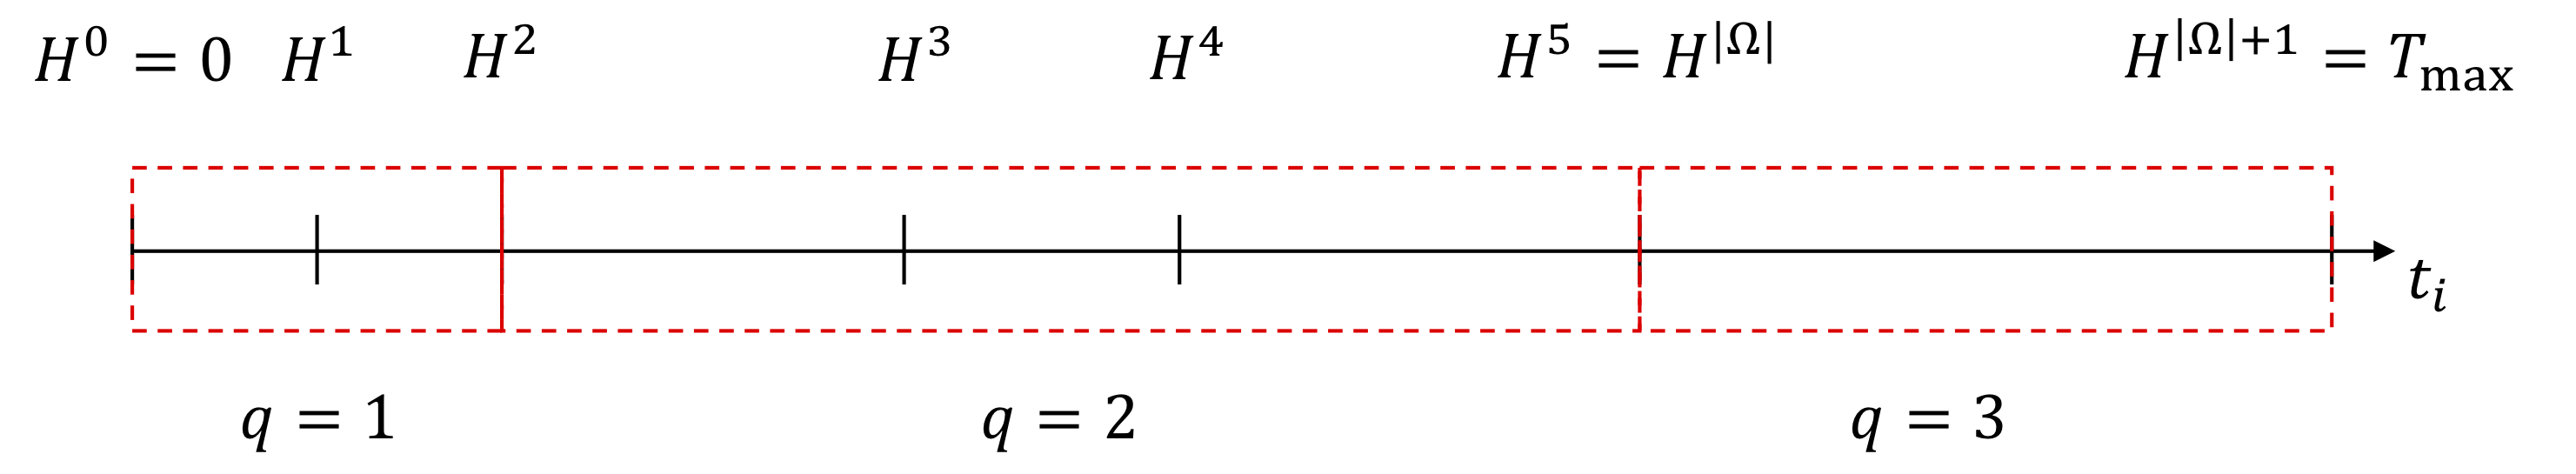
\includegraphics[width=0.8\textwidth]{simplePart}
		\caption{An illustration of partition on interval \([0,T_{\max}]\).}
		\label{fig:simplePart}
	\end{figure}
	\noi For each activity \(i \in I\), with the partition \(\mathcal{P}_i\) defined, we can see the starting time \(t_i\) of the master problem lies in the range specified by one element of \(\mathcal{P}_i\). We introduce an indicator \(y_i^q\), \(\forall i \in I, q \in \mathcal{Q}_i\) in the first stage:
	\begin{equation}
		y_i^q = \begin{cases}
			1 & \text{if \(t_i \in [H^{\underbar{\omega}^q},H^{\bar{\omega}^q}]\)}\\
			0 & \text{otherwise}
		\end{cases}
		\qquad \forall i \in I, q \in \mathcal{Q}_i,
	\end{equation}
	and we use the following constraints to represent this relationship:
	\begin{subequations} \label{cons:yCons}
		\begin{align}
			& \sum_{q \in \mathcal{Q}_i} H^{\underbar{\omega}^q} y_i^{q} \leq t_i \leq \sum_{q \in \mathcal{Q}_i} H^{\bar{\omega}^q} y_i^{q} \qquad \qquad \forall i \in I \label{cons:tyBounds}\\
			& \sum_{q \in \mathcal{Q}_i} y_i^q = 1 \qquad \qquad \forall i \in I. \label{cons:sumy1}
		\end{align}
	\end{subequations}
	In constraint~\eqref{cons:sumy1}, we enforce that \(t_i\) can only lie in one of the ranges specified by the partition, as only one of \(y_i^q\) can take value \(1\) for each \(i \in I\). Depending on the value of \(y_i^q\), we can write the bounds of the such range as in~\eqref{cons:tyBounds}. \\
	\newline
	The benefit of setting up the \(y\) variables is to obtain tighter bounds for \(t_i\) than the generic bounds \([0,T_{\max}]\) in Proposition~\ref{prop:bounds}. Suppose solving the master problem provides a solution \(\hat{y}_i^{\tilde{q}}, \forall i \in I, q \in \mathcal{Q}_i \). Then we can replace the big-\(M\) in constraints~\eqref{cons:sG1} and~\eqref{cons:sG2} of the scenario with moderate \(M_i^{\omega,+}\) and \(M_i^{\omega,-}\) because introducing variables \(y\) gives us better bounds on \(t_i\):
	\begin{subequations}
		\begin{align}
			& M_i^{\omega,+} = \sum_{q \in \mathcal{Q}_i} H^{\bar{\omega}^q} \hat{y}_i^q - H^\omega\\
			& M_i^{\omega,-} = H^\omega - \sum_{q \in \mathcal{Q}_i} H^{\underbar{\omega}^q} \hat{y}_i^q,
		\end{align}
	\end{subequations}
	and the constraints~\eqref{cons:sG1} and~\eqref{cons:sG2} become:
	\begin{subequations} \label{cons:newBoundsm}
		\begin{align}
			H^\omega + G_i \left(\sum_{q \in \mathcal{Q}_i} H^{\bar{\omega}^q} \hat{y}_i^q - H^\omega \right) \geq \hat{t}_i \qquad \qquad \forall i \in I\\
			H^\omega - (1 - G_i) \left(H^\omega - \sum_{q \in \mathcal{Q}_i} H^{\underbar{\omega}^q} \hat{y}_i^q \right) \leq \hat{t}_i \qquad \qquad \forall i \in I.
		\end{align}
	\end{subequations}
	The multiplication of \(G_i \hat{y}_i^q\) makes the dual of subproblem no longer linear of \(y\). To fix this, since \(\hat{y}_i^q\) is binary and \(G_i\) for all \(i \in I, q \in \mathcal{Q}_i\), we can introduce variables \(F_i^q\) to linearize the bilinear term and rewrite constraints~\eqref{cons:newBoundsm} as follows:
	\begin{subequations} \label{cons:newBoundsmlin}
		\begin{align}
			H^\omega + \sum_{q \in \mathcal{Q}_i} H^{\bar{\omega}^q} F_i^q - H^\omega G_i \geq \hat{t}_i \qquad \qquad \forall i \in I \label{cons:FG1}\\
			G_i H^\omega - \sum_{q \in \mathcal{Q}_i} H^{\underbar{\omega}^q} F_i^q \leq \hat{t}_i - \sum_{q \in \mathcal{Q}_i} H^{\underbar{\omega}^q} \hat{y}_i^q \qquad \qquad \forall i \in I \label{cons:FG2}\\
			F_i^q \leq G_i \qquad \qquad \forall i \in I, q \in \mathcal{Q}_i \label{cons:FGlin1}\\
			F_i^q \leq \hat{y}_i^q \qquad \qquad \forall i \in I, q \in \mathcal{Q}_i \label{cons:FGlin2}\\
			F_i^q \geq G_i + \hat{y}_i^q - 1 \qquad \qquad \forall i \in I, q \in \mathcal{Q}_i. \label{cons:FGlin3}
		\end{align}
	\end{subequations}
	In the subproblem, for each activity \(i \in I\), there is only one \(\hat{q} \in \mathcal{Q}_i\) such that \(\hat{y}_i^{\hat{q}} = 1\), which means \(\hat{t}_i \in [H^{\underbar{\omega}^{\hat{q}}},H^{\bar{\omega}^{\hat{q}}}]\). We examine the validity and effectiveness result of these tightened constraints. For validity, we check if constraints~\eqref{cons:newBoundsm} matches the logic when \(G_i\) is binary, while for effectiveness, we need to compare the feasible range of \(G\) in constraints~\eqref{cons:Grange} and that specified by constraints~\eqref{cons:newBoundsm}. \\
	\newline
	For a specific \(i \in I\), constraints~\eqref{cons:newBoundsm} can be rewritten using \(\hat{q}\):
	\begin{subequations} \label{cons:sGnew}
		\begin{align}
		H^\omega + G_i \left( H^{\bar{\omega}^{\hat{q}}} - H^\omega \right) \geq \hat{t}_i \label{cons:sGnew1}\\
		H^\omega - (1 - G_i) \left(H^\omega - H^{\underbar{\omega}^{\hat{q}}} \right) \leq \hat{t}_i. \label{cons:sGnew2}
		\end{align}
	\end{subequations}
	For a scenario \(\omega \in \Omega\), there are three possible positions of \(H^\omega\) relative to this range with \(\hat{y}_i^{\hat{q}} = 1\): \(H^\omega \in [H^{\underbar{\omega}^{\hat{q}}},H^{\bar{\omega}^{\hat{q}}}]\), \(H^\omega < H^{\underbar{\omega}^{\hat{q}}}\), or \(H^\omega > H^{\bar{\omega}^{\hat{q}}}\). When \(G_i = 1\), the left-hand side of constraint~\eqref{cons:sGnew1} is \(H^{\bar{\omega}^{\hat{q}}}\) and the left-hand side of constraint~\eqref{cons:sGnew2} is \(H^\omega\). When \(G_i = 0\), the left-hand side of constraint~\eqref{cons:sGnew1} is \(H^\omega\), and the left-hand side of constraint~\eqref{cons:sGnew2} is \(H^{\underbar{\omega}^{\hat{q}}}\).
	\begin{enumerate}
		\item 
			\(H^\omega \in [H^{\underbar{\omega}^{\hat{q}}},H^{\bar{\omega}^{\hat{q}}}]\): we can see that if \(\hat{t}_i \geq H^\omega\), by logic \(G_i\) should take value \(1\). Constraints~\eqref{cons:sGnew} match \(\hat{t}_i \geq H^\omega\) for \(G_i = 1\) and is violated for \(G_i = 0\). Similar validity results hold if \(\hat{t}_i < H^\omega\). In addition, the possible value \(G_i\) can take changes from the one shown in~\eqref{cons:Grange} to:
			\begin{equation*}
			\left(\hat{t}_i - H^\omega \right)/\left( H^{\bar{\omega}^{\hat{q}}} - H^\omega \right) \leq G_i \leq (\hat{t}_i - H^\omega)/\left(H^\omega - H^{\underbar{\omega}^{\hat{q}}} \right) + 1
			\end{equation*}
			Since the value of \(M\) decreases compared to constraints~\eqref{cons:Grange}, when \(\hat{t}_i \geq H^\omega\), the lower bound increases and upper bound is \(1\). When \(\hat{t}_i < H^\omega\), the upper bound decreases and the lower bound is \(0\). Therefore, the feasible range of \(G_i\) for each \(i \in I\) shrinks, which achieves the goal to tighten the subproblem relaxation.
		\item 
			\(H^\omega < H^{\underbar{\omega}^{\hat{q}}}\): we can see \(G_i = 1\) is feasible and \(G_i = 0\) violates constraint~\eqref{cons:sGnew1}. The possible value \(G_i\) can take becomes:
			\begin{align*}
			G_i \geq \left(\hat{t}_i - H^\omega \right)/\left( H^{\bar{\omega}^{\hat{q}}} - H^\omega \right)\\
			G_i \geq (\hat{t}_i - H^\omega)/\left(H^\omega - H^{\underbar{\omega}^{\hat{q}}} \right) + 1.
			\end{align*}
			Similar to Case 1, the lower bound increases compared to using a large \(M\) and the upper bound is \(1\), and we achieve a tightened relaxation.
		\item 
			\(H^\omega > H^{\bar{\omega}^{\hat{q}}}\): we can see \(G_i = 0\) is feasible and \(G_i = 1\) violates constraint~\eqref{cons:sGnew2}. The possible value \(G_i\) can take becomes:
			\begin{align*}
			G_i \leq \left(\hat{t}_i - H^\omega \right)/\left( H^{\bar{\omega}^{\hat{q}}} - H^\omega \right)\\
			G_i \leq (\hat{t}_i - H^\omega)/\left(H^\omega - H^{\underbar{\omega}^{\hat{q}}} \right) + 1.
			\end{align*}
			Similar to Case 1, the upper bound decreases compared to using a large \(M\) and the lower bound is \(0\), and we achieve a tightened relaxation.
	\end{enumerate}
	The tightened constraints~\eqref{cons:newBoundsm} is shown to have validity and effectiveness properties. However, for the latter two situations, \(H^\omega < H^{\underbar{\omega}^{\hat{q}}}\) and \(H^\omega > H^{\bar{\omega}^{\hat{q}}}\), \(G_i\) can still take fractional value. We further tighten the formulation by adding two constraints involving \(y\), such that if the subproblems belonging to those two situations, \(G_i\) can be fixed as either \(0\) or \(1\). For scenario \(\omega \in \Omega\), suppose solving the master problem provides the solution \(\hat{y}_i^q, \forall i \in I, q \in \mathcal{Q}_i\), we have:
		\begin{equation}\label{cons:subyG}
			\sum_{q \in \mathcal{Q}_i, H^\omega \leq H^{\underbar{\omega}^q}} \hat{y}_i^q \leq G_i \leq 1 - \sum_{q \in \mathcal{Q}_i, H^\omega \geq H^{\bar{\omega}^q}} \hat{y}_i^q \qquad \forall i \in I 
		\end{equation}
	Again we check the validity and the effectiveness result of constraints~\eqref{cons:subyG} for the three situations listed above:
	\begin{enumerate}
		\item 
			\(H^\omega \in [H^{\underbar{\omega}^{\hat{q}}},H^{\bar{\omega}^{\hat{q}}}]\): the lower bound is \(0\) since \(y_i^q = 0\) for all elements of partition left of \(\hat{q}\), and the upper bound is \(1\) because \(y_i^q = 0\) for all elements of partition right of \(\hat{q}\). Therefore, \(0 \leq G_i \leq 1\) is valid.
		\item 
			\(H^\omega < H^{\underbar{\omega}^{\hat{q}}}\): the lower bound is \(1\) since the summation term, \(\sum_{q \in \mathcal{Q}_i, H^\omega \leq H^{\underbar{\omega}^q}} \hat{y}_i^q\), includes \(y_i^{\hat{q}}\), which forces \(G_i = 1\). This matches the logic since \(\hat{t}_i \geq H^\omega\).
		\item 
			\(H^\omega > H^{\bar{\omega}^{\hat{q}}}\): the upper bound is \(1\) since the summation term, \(\sum_{q \in \mathcal{Q}_i, H^\omega \geq H^{\bar{\omega}^q}} \hat{y}_i^q\), includes \(y_i^{\hat{q}}\), which forces \(G_i = 0\). This matches the logic since \(\hat{t}_i \leq H^\omega\).
	\end{enumerate}
	With the addition of constraints~\eqref{cons:newBoundsmlin} and~\eqref{cons:subyG} in the subproblems, we present the tightened version of subproblems as follows: 
	\begin{subequations}
		\label{prob:subTightened}
		\begin{align}
		(S_{\mathcal{P}}^\omega) \qquad g^\omega_{\mathcal{P}}(\hat{t},\hat{x},\hat{y}) = \min \quad & t_T \\
		\text{s.t.} \quad & H^\omega + \sum_{q \in \mathcal{Q}_i} H^{\bar{\omega}^q} F_i^q - H^\omega G_i \geq \hat{t}_i \qquad \qquad \forall i \in I \label{cons:sFG1t}\\
		& G_i H^\omega - \sum_{q \in \mathcal{Q}_i} H^{\underbar{\omega}^q} F_i^q \leq \hat{t}_i - \sum_{q \in \mathcal{Q}_i} H^{\underbar{\omega}^q} \hat{y}_i^q \qquad \qquad \forall i \in I \label{cons:sFG2t}\\
		& F_i^q \leq G_i \qquad \qquad \forall i \in I, q \in \mathcal{Q}_i \label{cons:sFGlin1t}\\
		& F_i^q \leq \hat{y}_i^q \qquad \qquad \forall i \in I, q \in \mathcal{Q}_i \label{cons:sFGlin2t}\\
		& F_i^q \geq G_i + \hat{y}_i^q - 1 \qquad \qquad \forall i \in I, q \in \mathcal{Q}_i. \label{cons:sFGlin3t}\\
		& G_i \geq \sum_{q \in \mathcal{Q}_i, H^\omega \leq H^{\underbar{\omega}^q}} \hat{y}_i^q \qquad \qquad \forall i \in I \label{cons:syG1t}\\
		& G_i \leq 1 - \sum_{q \in \mathcal{Q}_i, H^\omega \geq H^{\bar{\omega}^q}} \hat{y}_i^q \qquad \qquad \forall i \in I \label{cons:syG2t}\\
		& \text{Constraints~\eqref{cons:stG1}-\eqref{cons:subH}}\\
		& 0 \leq x_{ij} \leq 1 \qquad \qquad \forall \,i \in I, j \in J_i\\
		& 0 \leq z_{ij} \leq 1 \qquad \qquad \forall \,i \in I, j \in J_i\\
		& 0 \leq G_i \leq 1. \qquad \qquad \forall \,i \in I. \label{cons:G01t}
		\end{align}
	\end{subequations}
	Suppose we solve the subproblems \((S_{\mathcal{P}}^\omega)\) for every \(\omega \in \Omega\) and generate a linear cut indexed by \(\ell\), where coefficients \(\pi,\lambda\) and \(\gamma\) can be calculated based on the dual variables obtained:
	\begin{equation} \label{cons:cut}
		\theta^\omega \geq v^{\omega,\ell} + \sum_{i \in I} \pi_i^{\omega,\ell} (t_i - \hat{t}_i^{\ell}) + \sum_{i \in I} \sum_{j \in J_i} \lambda_{ij}^{\omega,\ell} (x_{ij} - \hat{x}_{ij}^{\ell}) + \sum_{i \in I} \sum_{q \in \mathcal{Q}^{\ell}_i} \gamma_{i,q}^{\omega,\ell} \left( y_i^{q} - \hat{y}_i^{q,\ell} \right).
	\end{equation}
	Since the subproblem is a linear relaxation, \(\theta^\omega\) is a lower approximation of \(f^\omega\) for the current partition. However, since the validity result depends on the current partition, the cut needs to be modified once the partition is updated to retain the validity result. We assume that the update only refines the partition for each \(i \in I\):
	\begin{definition} \label{definition:refinement}
		For two partitions \(\mathcal{P}^1_i\) and \(\mathcal{P}^2_i\), indexed by \(\mathcal{Q}^1_i\) and \(\mathcal{Q}^2_i\) respectively, where \(\mathcal{P}^2_i\) is a refinement of \(\mathcal{P}^1_i\), we have:
		\begin{equation*}
		\forall q^2 \in \mathcal{Q}^2_i, \exists q^1 \in \mathcal{Q}^1_i \text{ s.t. } \bar{\omega}^{q^1} \geq \bar{\omega}^{q^2} \text{ and } \underbar{\omega}^{q^1} \leq \underbar{\omega}^{q^1}.
		\end{equation*}
	\end{definition}
	\noi Suppose at the current iteration for each \(i \in I\), the partition is \(\mathcal{P}_i\) indexed by \(\mathcal{Q}_i\), and this partition is updated from past partitions by only a sequence of refinement defined in Definition~\ref{definition:refinement}, cut~\eqref{cons:cut} can be updated to the following form so that the \(y\) variable has a proper dimension matching the current partition:
	\begin{align} \label{cons:updatedcut}
		& \theta^\omega \geq v^{\omega,\ell} + \sum_{i \in I} \pi_i^{\omega,\ell} (t_i - \hat{t}_i^{\ell}) + \sum_{i \in I} \sum_{j \in J_i} \lambda_{ij}^{\omega,\ell} (x_{ij} - \hat{x}_{ij}^{\ell}) + \nonumber \\
		& \qquad \sum_{i \in I} \sum_{\tilde{q} \in \mathcal{Q}^{\ell}_i} \gamma_{i,\tilde{q}}^{\omega,\ell} \left( \sum_{q \in \mathcal{Q}_i, H^{\bar{\omega}^{q}} \leq H^{\bar{\omega}^{\tilde{q},\ell}},H^{\underbar{\omega}^{q}} \geq H^{\bar{\omega}^{\tilde{q},\ell}} }y_i^{q} - \hat{y}_i^{\tilde{q},\ell} \right) \qquad \forall \ell = 1,2, \dots.
	\end{align}
	We show that, given a partition, \(\mathcal{P}\), which is updated from sequential refinement, \(\mathcal{P}^\ell, \ell = 1,2,\dots\), the cut~\eqref{cons:updatedcut} is a valid lower approximation for function \(g\):
	\begin{proposition} \label{prop:validity}
		Suppose we have a partition, \(\mathcal{P}\), which is indexed by sets \(\mathcal{Q}\), and the sequence of partitions, \(\{\mathcal{P}^\ell\}_{\ell = 1}\), each of which is indexed by sets \(\mathcal{Q}^\ell\). Assuming \(\mathcal{P}\) is a refinement of \(\mathcal{P}^\ell\) for every \(\ell = 1,2, \dots\), for any \(\omega \in \Omega\), we have
		\begin{align} \label{cons:validlb}
			&g^\omega_{\mathcal{P}}(t,x,y) \geq v^{\omega,\ell} + \sum_{i \in I} \pi_i^{\omega,\ell} (t_i - \hat{t}_i^{\ell}) + \sum_{i \in I} \sum_{j \in J_i} \lambda_{ij}^{\omega,\ell} (x_{ij} - \hat{x}_{ij}^{\ell}) + \nonumber \\ 
			& \qquad \qquad \sum_{i \in I} \sum_{\tilde{q} \in \mathcal{Q}^{\ell}_i} \gamma_{i,\tilde{q}}^{\omega,\ell} \left( \sum_{q \in \mathcal{Q}_i, H^{\bar{\omega}^{q}} \leq H^{\bar{\omega}^{\tilde{q},\ell}},H^{\underbar{\omega}^{q}} \geq H^{\bar{\omega}^{\tilde{q},\ell}} }y_i^{q} - \hat{y}_i^{\tilde{q},\ell} \right) \qquad \forall \ell = 1,2, \dots. 
		\end{align}
		at any given feasible \((t,x,y)\).
	\end{proposition}
	\begin{proof}
		We denote the recourse function corresponding to the partition \(\mathcal{P}^{\ell}\) as \(g^\omega_{\mathcal{P}^\ell}(t,x,y)\), where \(y\) has the correct dimension according to \(\mathcal{P}^\ell\). We first prove that 
		\begin{equation} \label{cons:gglb}
			g^\omega_{\mathcal{P}}(t,x,y) \geq g^{\omega}_{\mathcal{P}^\ell}(t,x,\tilde{y}) \qquad \forall \ell = 1,2,\dots
		\end{equation}
		where \[\tilde{y}_i^{\tilde{q}} = \sum_{q \in \mathcal{Q}_i, H^{\bar{\omega}^{q}} \leq H^{\bar{\omega}^{\tilde{q},\ell}},H^{\underbar{\omega}^{q}} \geq H^{\bar{\omega}^{\tilde{q},\ell}} }y_i^{q} \qquad  \forall i \in I, \tilde{q} \in \mathcal{Q}^\ell_i\]
		Suppose for an \(\omega \in \Omega\) and a \((t,x,y)\), we solve the problem \(S_{\mathcal{P}}^\omega\) and obtain the optimal solution \((t^{\omega,*},x^{\omega,*},G^{\omega,*},F^{\omega,*})\). It is easy to see that by transforming \(F^{\omega,*}\) to \(\tilde{F}^{\omega,*}\) with \[\tilde{F}^{\omega,*,\tilde{q}}_i = \sum_{q \in \mathcal{Q}_i, H^{\bar{\omega}^{q}} \leq H^{\bar{\omega}^{\tilde{q},\ell}},H^{\underbar{\omega}^{q}} \geq H^{\bar{\omega}^{\tilde{q},\ell}} }F_i^{\omega,*,q} \qquad  \forall i \in I, \tilde{q} \in \mathcal{Q}^\ell_i,\]
		we obtain a feasible solution \((t^{\omega,*},x^{\omega,*},G^{\omega,*},\tilde{F}^{\omega,*})\) to the recourse problem corresponding to the partition \(\mathcal{P}^\ell\). Therefore, inequality~\eqref{cons:gglb}. Furthermore, the cut generated at partition \(\mathcal{P}^\ell\) is
		\[\theta^\omega \geq v^{\omega,\ell} + \sum_{i \in I} \pi_i^{\omega,\ell} (t_i - \hat{t}_i^{\ell}) + \sum_{i \in I} \sum_{j \in J_i} \lambda_{ij}^{\omega,\ell} (x_{ij} - \hat{x}_{ij}^{\ell}) + \sum_{i \in I} \sum_{q \in \mathcal{Q}^{\ell}_i} \gamma_{i,q}^{\omega,\ell} \left( y_i^{q} - \hat{y}_i^{q,\ell} \right),\]
		 which means that for any feasible \((t,x,\tilde{y})\), we have 
		 \begin{equation} \label{cons:validglb}
		 	g^\omega_{\mathcal{P}^\ell}(t,x,\tilde{y}) \geq v^{\omega,\ell} + \sum_{i \in I} \pi_i^{\omega,\ell} (t_i - \hat{t}_i^{\ell}) + \sum_{i \in I} \sum_{j \in J_i} \lambda_{ij}^{\omega,\ell} (x_{ij} - \hat{x}_{ij}^{\ell}) + \sum_{i \in I} \sum_{q \in \mathcal{Q}^{\ell}_i} \gamma_{i,q}^{\omega,\ell} \left( \tilde{y}_i^{q} - \hat{y}_i^{q,\ell} \right).
		 \end{equation}
		 By substituting \(\tilde{y}\) by \(y\) and combining inequalities~\eqref{cons:gglb} and~\eqref{cons:validglb}, we obtain the result of~\eqref{cons:validlb}.
	\end{proof}
	\noi Proposition~\ref{prop:validity} states that if we perform a proper modification on the \(y\) variables to all cuts generated in the past, the modified cuts~\eqref{cons:updatedcut} will be a valid lower approximation for the current recourse function. Therefore, we incorporate the modified cuts~\eqref{cons:updatedcut} in our master problem, given a partition \(\mathcal{P}\) indexed by \(\mathcal{Q}\), which is shown as follows:
	\begin{subequations} \label{prob:masterTightened}
		\begin{align}
		(M_{\mathcal{P}}) \quad z_{\mathcal{P}}^* = \min \quad &p^0 t_T + \sum_{\omega \in \Omega} p^\omega \theta^{\omega}\\
		\text{s.t.} \quad & t_k - t_i \geq D_{i}(1 - \sum_{j \in J_i} x_{ij} e_{ij}) \qquad \qquad \forall \,i \in I, (i,k) \in \mathcal{A} \label{cons:MpSep}\\
		& \sum_{i \in I} \sum_{j \in J_i} b_{ij}x_{ij} \leq B  \label{cons:MpBudget}\\
		& \sum_{j \in J_i} x_{ij} \leq 1  \qquad \qquad \forall \,i \in I \label{cons:MpSingleBudget}\\
		& \sum_{q \in \mathcal{Q}_i} H^{\underbar{\omega}^q} y_i^{q} \leq t_i \leq \sum_{q \in \mathcal{Q}_i} H^{\bar{\omega}^q} y_i^{q} \qquad \qquad \forall i \in I\\
		& \sum_{q \in \mathcal{Q}_i} y^q_i = 1 \qquad \qquad \forall i \in I \label{cons:MpY1}\\
		& \theta^\omega \geq v^{\omega,\ell} + \sum_{i \in I} \pi_i^{\omega,\ell} (t_i - \hat{t}_i^{\ell}) + \sum_{i \in I} \sum_{j \in J_i} \lambda_{ij}^{\omega,\ell} (x_{ij} - \hat{x}_{ij}^{\ell}) \nonumber \\
		&\qquad + \sum_{i \in I} \sum_{\tilde{q} \in \mathcal{Q}^{\ell}_i} \gamma_{i,\tilde{q}}^{\omega,\ell} \left( \sum_{q \in \mathcal{Q}_i, \bar{H}_i^{q} \leq \bar{H}_i^{\ell,\tilde{q}},\underbar{H}_i^{q} \geq \underbar{H}_i^{\ell,\tilde{q}} }y_i^{q} - \hat{y}_i^{\tilde{q},\ell} \right) \nonumber \\
		& \qquad  \forall \omega \in \Omega, \ell = 1, 2, \dots\\
		& y_i^q \in \{0,1\} \qquad \qquad \forall i \in I, q \in \mathcal{Q}_i\\
		& t_i \geq 0 \qquad \qquad \forall \,i \in I\\
		& 0 \leq x_{ij} \leq 1 \qquad \qquad \forall \,i \in I, j \in J_i.
		\end{align}
	\end{subequations}
	We can see that if we keep refining the partition, the generated cuts will become tighter and we will be able to provide an improving lower bound as it progresses. The decomposition algorithm is presented as follows:
	\begin{algorithm}
		\caption{Decomposition algorithm to solve problem~\eqref{prob:extensive}}
		\label{alg:Cut}
		\begin{algorithmic}[1]
			\State Initialize with cut iteration number \(\ell = 0\), lower bound \(LB = 0\), upper bound \(UB = +\infty\), initial partition \(\mathcal{P}^\ell\) with its indexed set \(\mathcal{Q}^\ell\), and specified tolerance \(\epsilon > 0\) and \(\delta > 0\);
			\While{\(\frac{UB - LB}{UB} > \epsilon\)} 
			\State Solve master problem \((M_{\mathcal{P}})\) and obtain solution \(\hat{t}^{\ell}, \hat{x}^{\ell}, \hat{y}^{\ell}, \hat{\theta}^{\ell}\) and optimal value \(z_{P}^*\);
			\If{\(z_{P}^* > LB\)}
			\State Update \(LB = z_{P}^*\);
			\EndIf
			\State For each \(\omega \in \Omega\), solve problem \((S^\omega)\) and obtain \(f^{\omega}(\hat{t},\hat{x})\). 
			\State Calculate \(z^* = p^0 \hat{t}^\ell_T + \sum_{\omega \in \Omega} p^\omega f^{\omega}(\hat{t}^\ell,\hat{x}^\ell)\)
			\If{\(z^* < UB\)} 
			\State Update \(UB := z^*\) and record the best incumbent solution as \(t^* = \hat{t}^\ell, x^* = \hat{x}^\ell\) and \(y^* = \hat{y}^\ell\);
			\EndIf
			\State For each \(\omega \in \Omega\), solve problem \((S_{\mathcal{P}}^\omega)\) given \(\hat{t}^{\ell}, \hat{x}^{\ell}, \hat{y}^{\ell}, \hat{\theta}^{\ell}\) and obtain optimal value \(v^{\omega,\ell}\) and coefficients \(\pi^{\omega,\ell}, \lambda^{\omega,\ell}, \gamma^{\omega,\ell}\);
			\If{\(z^*_P < p^0 \hat{t}_T + \sum_{\omega \in \Omega} p^\omega v^{\omega,\ell} - \delta\)}
			\State Add the cuts of form~\eqref{cons:cut} to the master problem;
			\State Keep \(\mathcal{P}^{\ell + 1} = \mathcal{P}^\ell\) and \(\mathcal{Q}^{\ell + 1} = \mathcal{Q}^\ell\); 
			\State Update \(\ell = \ell + 1\);
			\Else
			\State Refine the partition and obtain the new partition \(\mathcal{P}^{\ell + 1}\) and its indexed sets \(\mathcal{Q}^{\ell + 1}\);
			\State Update \(\ell = \ell + 1\);
			\State Update the previously generated cuts in the master problem to the form of~\eqref{cons:updatedcut};
			\EndIf
			\vspace{0.1cm}
			\EndWhile{\textbf{end while}}
			\State Output \(UB\) as the optimal value of model~\eqref{prob:extensive}, and \(t^*, x^*,y^*\) as the optimal solution.
		\end{algorithmic}
	\end{algorithm}
	Finally we prove Algorithm~\ref{alg:Cut} converges in finite number of iterations. Since every partition update is a refinement and we have a finite set of scenario \(\Omega\), we can prove the finite convergence of Algorithm~\ref{alg:Cut} as long as with the finest partition we reach the optimum of problem~\eqref{prob:extensive}.
	\begin{proposition} \label{prop:finestPar}
		If a partition \(\hat{\mathcal{P}}\) has indexed sets \(\hat{\mathcal{Q}}\) and for each \(i \in I\), \(|\hat{\mathcal{Q}}_i| = |\Omega|\) and \(\bar{\omega}^q = \underbar{\omega}^q + 1,\ \forall q \in \hat{\mathcal{Q}}_i\), we have \[z^* = \min_{(t,x,y) \in \mathbb{X}}\ t_T + \sum_{\omega \in \Omega} g^\omega_{\hat{\mathcal{P}}}(t,x,y),\]
		where 
		\begin{equation*}
			\mathbb{X} = \left\{(t,x,y) \left| 
			\begin{aligned}
			& \eqref{cons:MpSep}-\eqref{cons:MpY1}\\ 
			&y_i^q \in \{0,1\} \qquad \forall i \in I, q \in \hat{\mathcal{Q}}_i\\
			& t_i \geq 0 \qquad \forall i \in I\\
			& 0 \leq x_{ij} \leq 1 \qquad \forall i \in I, j \in J_i
			\end{aligned}
			\right. \right\}.
		\end{equation*}
	\end{proposition}
	\begin{proof}
		First we can consider the subproblem \((S_\mathcal{P}^\omega)\) as a partial linear relaxation of the original extensive formulation. So \(z^* \leq z^*_\mathcal{P}\) is automatically true.\\
		\newline
		Next we prove that, given the partition in Proposition~\ref{prop:finestPar}, we can construct a feasible solution, \((t^*,x^*,G^*)\), to the extensive formulation~\eqref{prob:extensive} with the same objective value from the optimal solution, \((\hat{t},\hat{x},\hat{y})\), to the problem
		\[\min_{(t,x,y) \in \mathbb{X}}\ t_T + \sum_{\omega \in \Omega} g^\omega_{\hat{\mathcal{P}}}(t,x,y).\]
		Suppose for \(i \in I\), we denote the index of partition where \(y\) variable takes value \(1\) as \(q_i\). Since \(\bar{\omega}^q = \underbar{\omega}^q + 1,\ \forall q \in \hat{\mathcal{Q}}_i\), either \(q_i \in \{q \in \hat{\mathcal{Q}}_i \mid H^\omega \leq H^{\underbar{\omega}^q}\}\) or \(q_i \in \{q \in \hat{\mathcal{Q}}_i \mid H^\omega \geq H^{\bar{\omega}^q}\}\) is true. Thus, constraints~\eqref{cons:syG1t} and~\eqref{cons:syG2t} enforce that \(G_i\) in the problem \((S_{\hat{\mathcal{P}}}^\omega)\) takes binary value because the right-hand side expressions of those two constraints must be \(0\) or \(1\) simultaneously. This means that although subproblems are linear programs, the integrality is implied. Therefore, when we obtain the optimal solution \(\hat{G}^\omega\) from solving problems \((S_{\hat{\mathcal{P}}}^\omega)\) for each \(\omega \in \Omega\), solution \((\hat{t},\hat{x},\hat{G})\) will be feasible for the extensive formulation because \((\hat{t},\hat{x},\hat{y}) \in \mathbb{X}\) and \(G\) variables satisfy the constraints~\eqref{cons:stG1}-\eqref{cons:subH} and binary constraints. This result is equivalent to \(z_{\hat{\mathcal{P}}}^* \geq z^*\). Combining the results above we conclude that \(z^* = \min_{(t,x,y) \in \mathbb{X}}\ t_T + \sum_{\omega \in \Omega} g^\omega_{\hat{\mathcal{P}}}(t,x,y).\)
	\end{proof}
	\begin{theorem} \label{thm:converge}
		Algorithm~\ref{alg:Cut} terminates in finite number of iteration for any \(\epsilon \geq 0\). 
	\end{theorem}
	\begin{proof}
		From Proposition~\ref{prop:finestPar} we know that with the finest partition \(\hat{\mathcal{P}}\) where for each \(i \in I\), \(|\hat{\mathcal{Q}}_i| = |\Omega|\) and \(\bar{\omega}^q = \underbar{\omega}^q + 1,\ \forall q \in \hat{\mathcal{Q}}_i\), solving the problem \(\min_{(t,x,y) \in \mathbb{X}}\ t_T + \sum_{\omega \in \Omega} g^\omega_{\hat{\mathcal{P}}}(t,x,y)\) is equivalent to solving the extensive formulation. Since there are only finite number of scenarios, it takes finite number of steps of refinement to reach the finest partition. \\
		\newline
		For each subproblem, there is only a finite number of possible values of dual variables because each corresponds to one of the finitely many different bases. This means that, for any partition \(\mathcal{P}\), the recourse function \(g^\omega_{\mathcal{P}}\) can be represented by finitely many linear cuts. Therefore, in algorithm~\ref{alg:Cut}, only a finite number of cuts are added for a finite number of partitions before \(UB = z^*\) and \(LB = z^*_{\hat{\mathcal{P}}}\) is achieved, a.k.a. \(\frac{UB - LB}{UB} = 0\).
	\end{proof}
	\begin{comment}
	\textcolor{blue}{ The materials above are the most important idea I want to convey in this section. Here are some additional results we have discussed but I haven't compiled to \LaTeX \ yet. Time allowing, I can add some stuff in maybe tonight or this coming week.
		\begin{itemize}
			\item Concavity of \(\mathbb{E}_d \left[ f(x,H,d) | H \right]\) in \(d\).
			\item The analytical form of the recourse function when all \(d\) are \([0,1]\)-uniformly distributed, all \(D\) are equal, and the crashing option can only be integer.
			\item The recourse function is a decreasing function in terms of remaining budget, given the same remaining task set.
			\item Not optimal to delay the start of activity \(i\) unless there is no investment before \(i\), given a fixed \(H\).
			\item Only optimal to delay to a possible disruption time.
		\end{itemize}
	}
	\subsection{Parallel Networks}
		\begin{itemize}
			\item Not optimal to delay when \(d_i \geq 0\) if each branch only contains a single activity.
			\item If each branch is a serial path, it is possibly beneficial to delay the start of some activities.
		\end{itemize}
	\subsection{Y Networks}
\section{Properties of the Sample Average Approximation Problem} \label{sec:consistency}
	\subsection{Cheat?}
	\subsection{Consistency and Convergence Results}
	\subsection{IID vs. Stratified Sampling}

	\subsection{Deterministic Counterparts}
		List the test results of INFORMS presentation. State the fact that the fully stochastic makes great improvement over its deterministic counterparts.
		
%\section{Stochastic Mixed Integer Program Extension}
\section{Conclusions} \label{sec:conclusions}
\end{comment}

\section{Experimental Results} \label{sec:results}
	\textcolor{blue}{Test results:
	\begin{itemize}
		\item Describe the test examples: where do they come from, number of nodes, how are they generated.
		\item Cite Sen's paper and describe the implementation.
		\item Results.
	\end{itemize}}

\bibliographystyle{plain}
\bibliography{PERT_Bib}

\end{document}